\documentclass[12pt]{article}

%\usepackage{algorithm2e}
%\usepackage{algorithmic} 
\usepackage{amsmath}
\usepackage{amsthm}
\usepackage{booktabs}
\usepackage{dcolumn} 
\usepackage{epstopdf}
\usepackage{fourier}
\usepackage{fullpage}
\usepackage{graphicx}
\usepackage{hyperref}
\usepackage{longtable} 
\usepackage{natbib}
\usepackage{rotating}
\usepackage{tabularx}
\usepackage{tikz} 
\usepackage{xcolor} 

\hypersetup{
  colorlinks = TRUE,
  citecolor=blue,
  linkcolor=red,
  urlcolor=black
}

\DeclareMathOperator*{\argmax}{\arg\!\max}

\newcommand{\starlanguage}{Significance indicators: $p \le 0.05:*$,
  .$p \le 0.01:**$ and $p \le .001:***$.}  

\newif\ifdraft

%\drafttrue % or 
\draftfalse

\ifdraft
\newcommand{\important}[1]{\textcolor{red}{\textbf{#1}}}
\usepackage{setspace}
%\doublespacing
\else
\newcommand{\important}[1]{#1}
\fi

\begin{document} 

\title{Peer-to-Peer Rental Markets: \\ Some Thoughts on the ``Sharing Economy''} 

\date{\today}

\author{John J. Horton \\ Leonard N. Stern School of Business \\ New
  York University\footnote{Author contact information, datasets and
    code are currently or will be available at
    \href{http://www.john-joseph-horton.com/}{http://www.john-joseph-horton.com/
    Thanks to Andrey Fradkin, Ramesh Johari, Arun Sundararajan, Samuel Fraiberger and Joe Golden for helpful discussions and comments.
}.}
  \and 
  Richard Zeckhauser \\ Harvard Kennedy School \\ Harvard University
}
\maketitle

% grep '\\important{' sharing.tex | sed 's/\\important{//g' | sed 's/}//g'
% Sarah Cannon ; Lawrence Summers
% http://blogs.hbr.org/2014/10/how-uber-and-the-sharing-economy-can-win-over-regulators/
% http://blogs.hbr.org/2013/01/from-zipcar-to-the-sharing-eco/

\begin{abstract} 
Recent technological advances and entrepreneurial efforts have created a number of new peer-to-peer rental markets in which owners can rent out their durable goods. 
We consider the emergence of such a market and determine the market clearing rental rate, the patterns of trade and the surplus unlocked for different types of consumers. 
Our analysis considers both a short-run, before consumers can revise their ownership decisions and a long-run, in which they can. 
A survey of consumers finds broad support for the modeling conventions used---namely that ownership is determined by a forward-looking evaluation of planned usage. \newline \newline 
\noindent JEL J01, J24, J3 
\end{abstract} 

% \begin{abstract}
% \noindent  

% where these costs are presumably far lower. 
% In this paper, we consider the emergence of a peer-to-peer rental market for a category of goods where a rental market previously did not exist. 
% We examine both the short-run, before consumers can revise their ownership decisions, and the long-run when they can.  
% When the rental market emerges, both owners and non-owners economize on their usage until the market clears. 
% Rental rates are increasing in consumer valuations, as a higher valuation increases demand or reduces supply among non-owners and owners, respectively. 
% If the pre-rental market excess capacity of owners exceeds the capacity demanded by non-owners, a glut is possible. 
% In the long-run, all consumers can revise their ownership decisions and when this occurs, the rental rate equals the product market purchase price and ownership does not depend on consumer valuation.  
% If the market-clearing short-run rental rate is above the purchase price, ownership will increase in the long-run.
% The fraction of consumers owning in the long-run is the population average usage rate.
% In the long-run and short-run rental markets, the unlocked social surplus is increasing in the valuation of former non-owners and decreasing in the valuation of owners, though both groups see welfare increase in both the long- and short-runs. 
% In the long-run P2P rental market a higher product market price is supportable, as owners can partially offset the purchase price through rental income. 
% Because long-run rental rates equal the purchase price and consumers derive consumption value from the good even without rental, firms are not competitive in the long-run rental market.  
% A survey of consumers finds broad support for the modeling conventions used---namely that ownership is determined by a forward-looking evaluation of planned usage and that ownership and rental are gross substitutes. 
% The survey also highlights the importance of usage predictability and granularity in determining ownership. 
% \newline \newline 
% \noindent JEL J01, J24, J3
% \end{abstract} 

\section{Introduction}
Owners in rental markets have traditionally been firms that own assets for the specific purpose of serving that rental market. 
Some renting out by consumer-owners occurred, but it was confined largely to expensive goods infrequently used by their owners, such as vacation homes and pleasure boats. 
More often, consumer-owned goods were shared among family and friends, without explicit payment. 
This characterization of rental markets is changing, as new technology focused companies create peer-to-peer (P2P) rental markets for much wider class of goods. 
These so-called ``sharing economy'' start-ups have created rental markets for houses, cars, boats, bicycles, tools, office space, cameras, parking spaces, and even clothes. 

The most prominent example of this new kind of rental market is Airbnb, which allows individuals to rent out spare bedrooms, apartments or even entire homes. 
Airbnb and platforms like it have been heralded by many, as they they promise to expand access to goods, diversify individual consumption, increase efficiency by increasing asset utilization and provide income to owners \citep{sundararajan2013zipcar}.
Aside from the business interest in these platforms---Airbnb alone has attracted nearly \$800 million in venture capital investment\footnote{\href{http://www.crunchbase.com/organization/airbnb}{http://www.crunchbase.com/organization/airbnb}}---these companies have also attracted policy interest, much of it negative. 
Critics charge that the primary competitive advantage of these platforms is the ability to duck costly regulations---regulations that often are intended to keep costs from being imposed on third-parties.\footnote{See \cite{horton2014tragedy} for a discussion of the externalities imposed by Airbnb-style subletting in rented apartments.}   

The emergence of P2P rental markets raises a number of questions. 
The first question is why are they arising now, given that the economic problem they are attempting to solve has long existed. 
We argue that a number of factors matter. 
Technological advances, such as the mass adoption of smart-phones and the falling cost of developing and running large web sites
is clearly important. 
However, P2P rental markets also borrow heavily from hard-won industrial experience in the design and management of online marketplaces that predate them.
In particular, recommender systems and reputation systems all emerged during the early days of electronic commerce and are now de rigeur in P2P rental markets.  
This knowledge allows P2P rental platforms to overcome---or at least ameliorate---market problems such as facilitating trust, lowering search costs and reducing moral hazard/adverse selection.  
We develop this argument in more depth and point out relevant works from the literature. 

In addition to the question of why P2P rental markets emerge, another class of questions is what form they will take and what are their key characteristics. 
For example, what determines the rental rate and the quantity exchanged in the P2P rental market? 
How much consumer surplus is ``unlocked'' by the P2P rental market and how is it distributed? 
How does the short-run rental rate---where existing owners rent to non-owners---differ from the long-run in which owners and non-owners alike can revise their ownership decision in light of the existence of a P2P rental market?  
What is the effect on total product market demand?

% Model description 
We introduce a model in which consumers decide whether to purchase a good based on their expected usage, conditional upon purchase. 
Consumers differ in their expected usage. 
We assume that there are two consumer types and that the high-types are the only ones that purchase the good initially.  
Even those that purchase the good do not use it 100\% of the time. 
When the P2P rental market first emerges, the owners can rent to non-owners.  

While we assume a purchase price that splits consumers into owners and non-owners, other configurations are possible, such as one where everyone owns the good and no one owns the good. 
There is a ``sweet spot'' product market price for the peer-to-peer rental market to work---it has to be high enough that there is a substantial pool of non-owners that value the good, but not so high that there is no one willing to rent because no one owns the good.\footnote{Of course, in the long-run ownership decisions can be revised, but it would be difficult for a P2P rental market to take off for some class of goods were ownership was already universal.}   

The short-run rental market does not necessarily clear: if pre-P2P rental excess capacity exceeds demand, there is a glut. 
In practice, the inherent transaction cost of bringing excess capacity to the market would provide a price floor.     
Assuming a positive rental rate, both owners and non-owners use the good as if they were renting the good at the market-clearing rental rate. 
For renters the reason is that they do face that rental rate; 
for owners, they now face a marginal opportunity cost of usage, which is also the rental rate. 
The rental rate is increasing in the valuation of the high-types, which reduces supply, and the valuation of the low-types, which increases demand. 

In addition to the short-run, we consider a long-run where owners and renters alike can revise their ownership decisions. 
If the short-run rental rate is below the purchase price, then ownership is less attractive, which will reduce \emph{purchase} demand for product; likewise a rental rate above the purchase price increases ownership and hence purchase demand.
In the long-run P2P equilibrium, the purchase price equals the rental rate.  
In the long-run P2P rental market, both high and low types receive the same utility from owning or renting, decoupling individual preference from ownership. 
In practice, consumer risk-aversion would likely still cause higher-value consumers to be the owners, since a fall-off in market demand can be better absorbed by them though own-consumption. 

The emergence of the P2P rental market is Pareto improving. 
The greatest gains are obtained when low-types have a valuation of the good close to that of the high-types. 
This suggests that the greatest surplus will come when differences in ownership are driven by income effects rather than, as in our model, tastes. 

The existence of a P2P rental market allows for a higher maximum price in a market, as it can generate positive demand for a good at prices for which even high-types would not buy without the possibility of rental. 
Unsurprisingly, product markets in which everyone buys the good before the emergence of the P2P rental market can only see purchase demand fall when the rental market emerges. 

In the model, we consider a single stylized, divisible ``good.''  
Different goods have radically different patterns of usage that would strongly affect how amenable they are to renting. 
For example, goods with predictable usage are far easier to rent out with little lost utility to the owner. 
Similarly, goods that are used in large chunks of time---with no use in between---are more amenable to rental to goods that have usage broken up into many small chunks of time. 
In the last part of the paper, we rely on survey evidence to explore what kinds of goods are particularly amenable to P2P rental as well as assess some of the assumptions of the model. 

Consumers were asked a series of questions about a single good (e.g., a BBQ grill) such as whether they own one, whether they have lent it out or borrowed it and, regardless of whether they own it, how much they would use it. 
If they do not own it, they were asked why. 
We also asked questions about how the good in question is characteristically used and how predictable that usage is
Finally, the respondent was asked for their household income.  

For only a small number of goods (e.g., vacation homes) is income important in determining ownership. 
For other goods, planned usage was primary the driver, supporting our basic modeling framework.  
We find that with cars excluded, there is a strong negative relationship between ownership and rental. 
Given that P2P rental markets are nascent, respondents are presumably renting from conventional rental companies, but it still supports the modeling view that non-owner does not imply zero value from usage. 

We conclude with some thoughts on how P2P rental markets might evolve.
Our analysis has focused on a single homogeneous good, but a key advantage of P2P rental markets might be in facilitating greater consumption diversity. 
In addition to whatever direct utility this diversification provides, it might also increase the stock of people with direct experience with a particular good, which combined with the continued proliferation of consumer-generated reviews and ratings might stimulate quality improvements. 
In that same vein, we also discuss how the producers of goods might react to P2P rental markets. 
In particular, they might modify goods to make them more or less amenable to rental, depending on their own market power. 
One issue we have largely ignored but which is potentially very important is that in many P2P rental markets owners also provide a labor input.
We discuss how this might be modeled and what the implications might be. 
Lastly, we sketch out some areas for future research. 
 
\section{Factors in explaining the rise of peer-to-peer rental markets}

The somewhat obvious economic rationale for P2P rental markets is that most durable goods are used by their owners far less than 100\% of the time, and the excess capacity this under-utilization generates could be rented out.
The demand side in such a market would be non-owners that still value the good.\footnote{
A non-owner might mean a non-owner in a particular place and time. 
Many Airbnb guests own homes---they just don't own homes everywhere. 
} 
These kinds of exchanges between consumers have always been technically possible, but transaction costs were prohibitive. 

Any potential P2P rental markets would have the typical transaction costs, such as finding and evaluating trading partners.
But informational problems are not the sole reason P2P rental markets were missing---individuals also simply lack the resources of firms that make commercial transactions feasible. 
Individuals lack marketing budgets, ways of accepting payments that are convenient for customers, standard contracts and procedures to draw upon, well-adapted insurance products, procedures and facilities for re-setting goods after use and so on. 
Because of both the lack of resources and the inherent information problems, consumer-owned goods have historically just been truly shared been between family members and neighbors rather than strangers, except when the potential gains from trade are sufficiently large (such as in the example of vacation home and boat rentals). 

P2P rental markets have emerged as entrepreneurs have taken advantage of technological advances to build facilitating platforms. 
The platforms lower transaction costs and provide individual owners tools previously only available to the firm. 
The maturation and increasing penetration of the Internet and the proliferation of smart phones, high resolution cameras and so on---were the technological shock that made these P2P rental markets feasible. 
However, these P2P rental markets have also stood on the shoulders of their electronic commerce predecessors, such as eBay, that made strides towards solving some of the problems inherent to online market places. 

Like all software companies, platforms have benefited from the rise of the Internet, which has radically increased the supply of potential users on both sides of the markets. 
They have also benefited from improving industrial knowledge about how to build and maintain large websites.
The cost of creating such sites has also fallen dramatically. 

A key challenge in all markets is facilitating trust among strangers, and this problem is even more acute in P2P rental markets, given the ``opportunity'' renters have to destroy or misuse the owner's capital.  
Facilitating trust is not a solved problem in online markets, but the experiences of early electronic commerce pioneers such as eBay provided2P rental market entrepreneurs a number of ready-made solutions to market problems related to trust. 
For example, every P2P rental market we are aware of uses some modified version of eBay's successful bi-lateral reputation system. 
The flaws in early versions of these systems---such as the ability for parties to condition their feedback on their trading partner's feedback---also clearly influenced the design of follow-on systems used in P2P rental markets. 
The rise of social networks such as Facebook has given platforms new opportunities to inject information into the the platform that parties can use in their decision-making. 

Online markets in general lack many of the market-thickening coordination mechanisms available in offline markets such as time and geography.
For example, buyers and sellers of vegetables benefit from agreeing that the Union Square green market is located in the northwest side of the Union Square Park and is open Mondays from 8:00 a.m. - 6:00 p.m.
The adaptation in the online world has been partially to create taxonomies and extensive classification of goods, but another approach has been to rely more on algorithmic innovations such as search algorithms and recommendation systems \citep{resnick1997recommender, adomavicius2005toward}.
These kids of approaches are particularly important in P2P rental markets because the goods being rented are often highly differentiated, as our consumer preferences, making matching more important. 

In addition to simply finding each other, would-be trading partners must asses the each other and the goods being traded. 
Verifiable measurements can often overcome some of the information problems in markets, and as \cite{varian2010computer} points out, advances in information technology are often advances in measurement. 
Consider that Uber is only possible because both sides of the market now carry with them taximeters (when running the appropriate software) at all times: 
a smart-phone with GPS technology allows for the precise measures of distance traveled.
In fact, this computer-mediated approach works even better than the traditional taximeter in that both parties can verify that the best route was taken. 
The proliferation of high-resolution digital cameras built into smart-phones have similarly made it easier for parties to inspect goods ex ante (Airbnb in particular benefits from this innovation).  
 
In terms of capacity, platforms do many of the things that individual owners would find costly. 
For example, they handle credit card payments. 
They create tools for ``self-serve'' marketing (such as through attractive profile pages) and through general platform marketing to bring renters to the platform. 
They also create software tools that let owners manage their availability, learn about the attributes of potential renters and so on. 


% \begin{table} 
% \begin{tabular}{lll}
% Airbnb     & Lodging & \\ 
% RelayRides & Transportation & \\ 
% Boats      &  & \\ 
% Equipment  &  & \\ 
% \end{tabular} 
% \end{table} 

\section{Model}

This assumption that consumers must consider the time required to use a good in making their consumption plan is similar in spirit to \cite{becker1965theory}; the possibility of sharing a good is similar in spirit to \cite{varian2000}.
Varian in particular discusses---in the context of information goods---how planned usage affects the rent-versus-own decision. 

\subsection{Consumer decision about ownership based on expected usage}  
Every consumer has a unit of time to allocate to various activities, some of which involve the usage of a good.  
Consumers have to decide how much time, $x \in [0,1]$, to devote to using a particular good. 
There is decreasing marginal utility from usage from a good: 
the consumer receives a benefit of $2\alpha x$, but as also a cost $c(x) = x^2$,  
where $\alpha \in (0,1)$ parametrizes their valuation of the good. 
The consumer's utility for a given $x$ is 
\begin{align}
u(x) = 2 \alpha x - x^2,  
\end{align} 
and so individual usage conditional upon owning the good is $x^* = \alpha$ and indirect utility is 
\begin{align}
v(\alpha) = u(x^*) = \alpha^2.  
\end{align} 
The purchase price of the good is $p$ and so a consumer will buy the good only if $\alpha^2 > p$. 
Note that for all $\alpha^2 > p$, the consumer will have an amount of time $1 - x^*$ when they are not using the good.
This is what they will be able to rent out---plus however much more capacity becomes available when they economize their own usage in light of the market clearing rental rate---when the P2P rental market emerges. 

Figure~\ref{fig:consumer} illustrates the consumer problem, showing the utility from various levels of usage depending on consumers with different values of $\alpha$.
The usage solution for each consumer is their $\alpha$ parameter and since indirect utility is just $\alpha^2$, the optimal usage for each value falls along the curve traced out by $x^2$.
The purchase price $p$ determines who buys the good, with all those having $\alpha^2 > p$ deciding to own and those below choosing not to purchase the good. 

\pgfmathsetmacro{\alphaOne}{0.40}
\pgfmathsetmacro{\xstarOne}{\alphaOne}%
\pgfmathsetmacro{\ustarOne}{2*\alphaOne * \alphaOne - \alphaOne^2}%

\pgfmathsetmacro{\alphaTwo}{0.55}
\pgfmathsetmacro{\xstarTwo}{\alphaTwo}%
\pgfmathsetmacro{\ustarTwo}{2*\alphaTwo * \alphaTwo - \alphaTwo^2}%

\pgfmathsetmacro{\alphaThree}{0.75}
\pgfmathsetmacro{\xstarThree}{\alphaThree}%
\pgfmathsetmacro{\ustarThree}{2*\alphaThree * \alphaThree - \alphaThree^2}%

\begin{figure}
\caption{Consumer purchase problem}
\label{fig:consumer} 
\begin{center}
\begin{tikzpicture}[scale=5]
\draw (1,0) node[below]{$x$} -- (0,0) --(0,1) node[left]{$u$};
\draw[thick, domain=0:0.98] plot (\x, {2.0 * \alphaOne *\x - \x*\x});
\node[align=right] at (1, 2.0 * \alphaOne - 1){$\alpha = \alphaOne$};
\draw[dotted] (\xstarOne, 0.0) to (\xstarOne, \ustarOne);

\draw[thick, domain=0:0.95] plot (\x, {2.0 * \alphaTwo *\x - \x*\x});
\node[align=right] at (1, 2.0 * \alphaTwo - 1){$\alpha = \alphaTwo$};
\draw[dotted] (\xstarTwo, 0.0) to (\xstarTwo, \ustarTwo);

\draw[thick, domain=0:0.95] plot (\x, {2.0 * \alphaThree *\x - \x*\x});
\node[align=right] at (1, 2.0 * \alphaThree - 1){$\alpha = \alphaThree$};
\draw[dotted] (\xstarThree, 0.0) to (\xstarThree, \ustarThree);

\draw[thick, dotted, domain=0:0.95] plot (\x, {\x*\x});

\draw[ultra thick] (0, 0.35) to (1, 0.35) node[right]{$p$}; 

\node[align=left] at (1, 1){$u(x^*) = \alpha^2$};

\draw[<->, red, ultra thick] (1.2,0)  -- (1.2, 0.35) ;
\node[red, align = left] at (1.5, 0.17) {Consumer\\does\\not\\buy};

\draw[<->, green, ultra thick] (1.2,0.35)  -- (1.2, 1) ;
\node[green, align = left] at (1.5, 0.65) {Consumer\\buys};
\end{tikzpicture}
\end{center}
\end{figure} 

\subsection{Three consumption possibilities with two consumer types} 
Consider a marketplace with two consumer types that are equally common: $\alpha_H$ and $\alpha_L$ with $\alpha_H > \alpha_L$. 
For a given price $p$, there are three market possibilities: 
when $\alpha_L^2 > p$ everyone buys the good; when $\alpha_H^2 > p > \alpha_L^2$, high-types buy the good but low-types do not; when $\alpha_H^2 < p$  no one buys the good. This gives a market demand curve of 
\begin{align}
   D(p) = \left\{
     \begin{array}{ll}
       0 & : p > \alpha_H^2\\
       1 & : \alpha_H^2 \ge p > \alpha_L^2  \\
       2 & : p \le \alpha_L^2  \\
     \end{array}
   \right.
\end{align} 

The three market possibilities are shown in Figure~\ref{fig:three_types}. 
The figure shows the space defined by $\alpha_H \in [0,1] \times \alpha_L \in [0,1]$ when $p = \frac{1}{2}$.
Since $\alpha_H > \alpha_L$ by definition, we only consider the space above the 45 degree line. 
The upper-right triangle labeled ``Both buy'' is the region where both consumer-types buy and the lower-left triangle where neither buy.  
This area is defined by $\alpha_L^2 > p$ and $\alpha_H^2 > p$. 
To show the geometry of the problem, the square of the valuation parameter is plotted in a faint dotted line; 
the associated minimal-but-still-purchasing valuation parameter is shown as $\underline{\alpha}_H$ and $\underline{\alpha}_L$ for the high- and low-types, respectively. 
The upper left rectangle shows the region where the high-types buy but the low-types do not, while the lower left triangle shows the region where neither buy. 
We are particularly interested in the rectangle where high-types buy but low-types do not, because in this region, the purchasing high-types have excess capacity, $\alpha_H < 1$, but the low-types still value usage of the good, $\alpha_L > 0$, despite their non-purchase. 
In this region, the immediate possibility of mutually beneficial trade exists between the two types, whereas in the other spaces a revision in the ownership decision is needed to support a P2P rental market. 

\newcommand*{\p}{0.30}%
\pgfmathsetmacro{\alphaMin}{sqrt{\p}}%
\pgfmathsetmacro{\neitherY}{(\p + 1.3*sqrt(\p))/2}%
\pgfmathsetmacro{\neitherX}{\p}%
\pgfmathsetmacro{\highY}{(1.3 + sqrt(\p))/2}%
\pgfmathsetmacro{\highX}{\p}%
\pgfmathsetmacro{\bothY}{(\alphaMin + 1.4)/2}%
\pgfmathsetmacro{\bothX}{(\alphaMin + 0.9)/2}%

\newcommand{\baseMarket}{
\draw (1,0) node[below]{$\alpha_L$} -- (0,0) --(0,1) node[left]{$\alpha_H$};
\draw (1,0) -- (1,1); 
\draw[dotted, domain=0:1] plot (\x, {\x * \x});

% \draw[dotted, domain=0:1] plot (\x, {sqrt{\x}});


\draw[dotted] (\p, 0) node[below] {$p$} to (\p, \alphaMin); 
\draw[dotted] (0, \p) node[left] {$p$} to (\alphaMin,\p);
\draw[thick] (0, \alphaMin) node[left]{$\underline{\alpha}_H$} to (\alphaMin, \alphaMin); 
\draw[dotted] (\alphaMin,0) node[below]{$\underline{\alpha}_L$} to (\alphaMin,\alphaMin);
\draw[thick] (\alphaMin,\alphaMin) to (\alphaMin,1);
\draw[ultra thick] (0,0) -- (\alphaMin, \alphaMin) -- (0, \alphaMin) -- (0,0);  % Neither
\draw[ultra thick] (0,\alphaMin) -- (\alphaMin, \alphaMin) -- (\alphaMin, 1) -- (0,1) -- (0,\alphaMin);  % high-types
\draw[ultra thick] (\alphaMin,\alphaMin) -- (\alphaMin, 1) -- (1, 1) --  (\alphaMin,\alphaMin);  % both
\node[align=left, below] at (\neitherX, \neitherY){Neither\\own};
\node[align=left, below] at (\highX, \highY){High-types\\own};
\node[align=left, below] at (\bothX, \bothY){Both\\own};
\node[align=right, right] at (1,1){$(1,1)$};
\node[align=right, left] at (0,0){$(0,0)$};
}
 
\begin{figure}
\caption{Three consumer market possibilities in the absence of P2P rental with two consumer types}
\label{fig:three_types} 
\begin{center}
\begin{tikzpicture}[scale=6]
\baseMarket
\end{tikzpicture}
\end{center}
\end{figure} 

\subsection{Short-run P2P rental market equilibrium} 
We now suppose that through some technological advance, it becomes possible for the high-types to costlessly rent their entire excess capacity to the low-types. 
As first, we will assume that no one can revise their original ownership decisions in light of this advance. 
Call the resulting equilibrium the ``short-run.'' 
Before the possibility of rental, the high-types were simply consuming $\alpha_H$, giving $1-\alpha_H$ to rent out.
If they had purchased the good, the low-types would consume $\alpha_L$. 
However, with the new possibility of rental, each consumer's decision problem has changed. 
The new owner optimization problem is 
\begin{align}
\argmax_x \quad 2\alpha_H x - x^2 -p + \underbrace{(1-x)r}_{\mbox{{\tiny Rental income}}},   \nonumber 
\end{align} 
whereas the renter optimization problem is 
\begin{align}
\argmax_x \quad 2 \alpha_L x - x^2 - \underbrace{xr}_{\mbox{{\tiny Rental cost}}},  \nonumber
\end{align} 
where $r$ is the taken-as-given rental rate. 
Assuming an interior solution (which requires that $2\alpha_L > r$), both decision problems yield the same usage decision, 
\begin{align}
x^*(\alpha_i) = \alpha_i - r/2. 
\end{align} 
where $i$ indexes consumer type. 
Let $x_H = x^*(\alpha_H)$ and $x_L = x^*(\alpha_L)$. 
For the rental market to clear $1 - x_H(r) = x_L(r)$.
If the market clears, then the rental rate is thus
\begin{align} \label{eq:strr} 
r = \alpha_H + \alpha_L - 1.  
\end{align} 
The quantity of the good exchanged is 
\begin{align}
Q = \frac{1}{2}\left(1 - \alpha_H + \alpha_L\right). 
\end{align} 
Note that if $1-\alpha_H > \alpha_L$, then a negative rental rate would be market clearing.
 
A negative rental rate arises when the owner's excess capacity in the absence of a rental market exceeds the non-owner's usage if given the good for free.
\important{If all consumers were allocated the good and their cumulative usage, $\alpha_H + \alpha_L$, exceeds the capacity of the actual stock of purchased goods, then a positive rental rate is needed to clear the market.}
Figure~\ref{fig:market_clearing} illustrates market clearing with a positive rental rate and the glut condition. 
The rental market demand is simply $x_L(r)$, whereas supply is $1-x_H(r)$. 
The market-clearing quantity is the optimal consumption of the low-types, $\alpha_L - r/2$. 
We add a supply curve with a lower $\alpha_H$ value (which moves out the supply curve, in red) such that the offered supply at $r = 0$ exceeds demand, creating a glut.  
\important{It is also clear from the figure that if the valuation parameter of either type rises, short-run rental rates increase, as increases in valuation lower supply and increase demand.} 
 
\newcommand*{\alphaH}{0.80}%
\newcommand*{\alphaL}{0.50}%
\newcommand*{\alphaHp}{0.40}
\pgfmathsetmacro{\r}{-1 + \alphaH + \alphaL}%
\pgfmathsetmacro{\Q}{\alphaL - \r/2}
\begin{figure} 
\caption{Market clearing with two consumer types in a P2P rental market} 
\label{fig:market_clearing} 
\begin{center}
\begin{tikzpicture}[scale = 6]
\draw[<->] (1,0) node[below]{$Qty$} -- (0,0) --(0,1) node[left]{$r$};
\draw[ultra thick] (1.0 - \alphaH, 0) to (1 - \alphaH + 0.5, 1.05) node [above] {$S(r) = 1 - x_H(r) = \alpha_H + r/2$};  
\draw[ultra thick, red] (1.0 - \alphaHp, 0) to (1 - \alphaHp + 0.50, 1.0) node [right] {$S_1(r) = 1 - \alpha_H' + r/2$};  
\draw[ultra thick] (\alphaL,     0) to (\alphaL - 1/2, 1) node [right]
{$D(r) = x_L(r) \alpha_L - r/2$}; 
\draw [dotted] (0, \r) node[left]{$r^*$} -- (\Q,\r) -- (\Q, 0) node[below]{$\alpha_L - r^*/2$}; % -- (\Q, 0);
\node[align=left, above, red] at (1, .15){Glut:\\ $S_1(0) > D(0)$; \\ $(1 - \alpha_H') > \alpha_L$}; 
\end{tikzpicture}
\end{center}
\end{figure} 

\subsection{Social Surplus in the P2P rental market short-run} 
With the introduction of the P2P rental market there are several welfare-affecting changes: 
high-type consumption goes down (from $x_H = \alpha_H$ to  $x_H = \alpha_H - r/2$) and low-type consumption goes up (from $x_L = 0$ to $x_L = \alpha_L - r/2$). 
Change in utility for the high-types from reduced consumption is 
\begin{eqnarray}
\Delta v_H &=& \underbrace{\left[2 \alpha_H \left(\alpha_H - r/2\right) - \alpha_H^2 \right]}_{\mbox{New P2P consumption utility}} - 
                             \underbrace{\left[\alpha_H^2 \right]}_{\mbox{Old consumption utility}}   \notag \\
           &=& - \frac{r^2}{4}. 
\end{eqnarray} 
This is negative, but it is compensated by the rental income. 
The greater the rental rate, the greater the loss in utility from reduced consumption. 
For the low-types, the change in utility from increased consumption is
\begin{align}
\Delta v_L = \alpha_L^2 - \frac{r^2}{4}. 
\end{align} 
The total change in consumer surplus from the introduction of the P2P rental market is thus: 
\begin{align}
\Delta S &= \Delta v_H + \Delta v_L \notag \\ 
         &=  \alpha_L^2 - \frac{r^2}{2} \notag \\
         &= \alpha_L^2 - \frac{1}{2} \left( \alpha_H + \alpha_L -1 \right)^2.
\end{align} 
Figure~\ref{fig:welfare} is a contour plot of change in social surplus from the emergence of the P2P rental market for the space of possible valuation parameters.
The figure shows what we might already intuit: higher values of $\alpha_L$ increase the gain in social surplus.
Indeed, $\partial \Delta S/\partial \alpha_L = 1 - \alpha_H + \alpha_L > 0$ since $\alpha_H < 1$ and $\alpha_L > 0$. 
\important{The more the non-owners value the good, the greater the increase in social surplus from the emergence of P2P rental markets.} 
The case of $\alpha_H$ is more complex. 
Recall that a positive rental rate only occurs when $\alpha_H + \alpha_L > 1$.
\important{As such, an increase in the valuation of the high-types reduces social surplus from P2P rental markets in non-glut P2P rental scenarios:   
\begin{align} 
\frac{\partial \Delta S}{\partial \alpha_H} =  1 - (\alpha_H + \alpha_L) < 0.
\end{align}} 
In Figure~\ref{fig:welfare} the line stretching from $(1,0)$ to $(1/2, 1/2)$ indicates the glut/non-glut boundary. 
For all points to the right of that line, a higher $\alpha_H$ valuation reduces social surplus.  
As, such the greatest social surplus is ``unlocked'' by the emergence of the P2P rental market when both purchasers and non-purchasers have similar, high valuations. 
In terms of the figure, the highest obtainable social surplus values for a fixed $\alpha_H + \alpha_L$ run along the 45 degree line that indicates $\alpha_H \approx \alpha_L$. 

For simplicity, we have ignored income effects as a cause of the pattern of ownership. 
However, for goods where income effects are important in the consumer's ownership decision problem, the $\alpha_H > \alpha_L$ requirement would no longer hold and potentially larger gains in social surplus would be unlocked by the P2P rental market emergence. 

\begin{figure}
\centering 
\caption{Consumer welfare as a function of high- and low-type consumer valuations}
\label{fig:welfare}
\begin{minipage}{0.50 \linewidth}
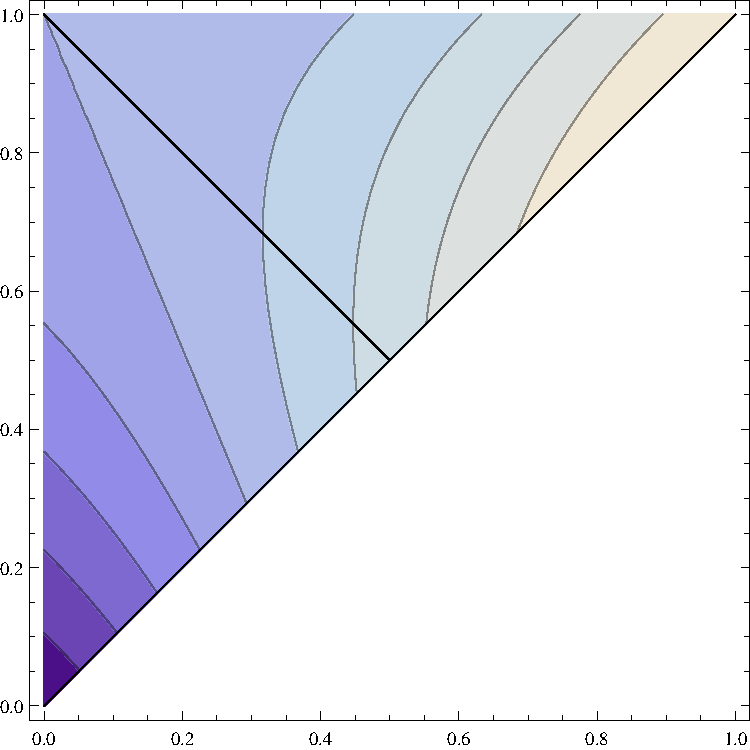
\includegraphics[width = \linewidth]{./plots/welfare.pdf}
\end{minipage} 
\end{figure} 

\subsection{Long-run P2P rental equilibrium} 
In the long-run equilibrium, all parties can revise their ownership decisions. 
The utility from owning is 
\begin{align}
v^{OWN}_i = 2\alpha_i x_i - x_i^2 + (1-x_i)r_{LR} - p   
\end{align} 
whereas the utility from renting is 
\begin{align}
v^{RENT}_{i} = 2\alpha_i x_i - x_i^2 - x_i r_{LR}  
\end{align} 
where $r_{LR}$ is the market-clearing long-run rental rate. 
The first order condition for either choice is $2 \alpha_i - 2 x_i - r_{LR} = 0$ and so $x^*_i = \alpha_i - r_{LR}/2$. 
Computing the indirect utility for both decisions, we have
\begin{align} 
v^{OWN} = \alpha_i^2 - p + \frac{r_{LR}^2}{4} + (1 - \alpha_i) r_{LR} \quad  \mbox{and} \quad v^{RENT} = \frac{1}{4} (r_{LR}- 2\alpha )^2. 
\end{align} 
Setting $v^{OWN} = v^{RENT}$ to find the conditions under which a user would be indifferent between renting and owning, the $\alpha_i$ term drops out and we are left with 
\begin{align}
p = r_{LR}. 
\end{align}
 \important{In the long-run P2P rental equilibrium, the rental rate equals the product market purchase price and ownership does not depend on usage patterns or valuation.}  

For this new market to clear, we have to determine what fraction of consumers choose to own. 
Let $f$ be the fraction of consumers that purchase the good in equilibrium. 
As ownership does not depend on valuation, we assume that both consumer types are equally likely to own. 
For the market to clear, 
\begin{align}
\left[ (1-x_H(p)) + (1-x_L(p))\right]f = \left(x_H(p) + x_L(p) \right)(1- f) 
\end{align} 
which simplifies to 
\begin{align}
f = \frac{x_H(p) + x_L(p)}{2}.  
\end{align} 
\important{The fraction of consumers owning in the long-run is the average usage rate in the population.}  
In this long-run P2P rental equilibrium, even though both types own, we might expect in practice for higher-valuation types to be the ones to own, as they can better bear the risk in the rental rate, ala \cite{sinai2005}.

In the long-run P2P rental market equilibrium, there are no profits from owning to simply rent-out, since the good costs $p$ and rental income is just $p$.  
However, owners and non-owners alike get a surplus. 
\important{This suggests that firms that derive no consumption value from the good can not compete in a competitive market: 
because the consumer has excess capacity after satisfying their own consumption, they can ``profitably'' sell their excess capacity at any price and still have positive utility; a firm owning simply to rent would make zero profit.} 
There is already perhaps some evidence that P2P rental markets are adversely affecting traditional firms: 
\cite{byers2013rise} find that Airbnb is already winning customers from hotels catering to the lower-end of the market. 
Firms do have other advantages over consumers, such as economies of scale or expertise in minimizing transaction costs. 
However, this firm-level expertise might simply be offered to consumers without the firm taking ownership.\footnote{A recently launched start-up called \href{https://www.guesty.com/}{Guesty} aims to be a kind of property management company for Airbnb rentals.} 

\subsection{Product market demand in the long-run P2P rental market equilibrium} 
Most commentators considering the sharing economy assume that sharing economy platforms reduce ownership. 
The intuitive idea is that there is a fixed amount demand for some good---a ``lump of consumption''---and that when idle goods are pulled into the market, demand can be met with a smaller total number of goods.
\important{This is not the case:  
ownership increases if the product market price is below the short-run rental rate.} 
Intuitively, when the short-run rental rate is greater than the purchase price, a consumer could buy the good at $p$ and rent out the entire capacity for $r$ and since $r > p$, earn a profit. 

To see this algebraically, first consider that in the long-run P2P equilibrium, the new product market demand curve, $D_1$, is
\begin{align}
D_1(p) &= 2f \notag \\  
     &= x_H(p) + x_L(p) \notag \\ 
     &= \alpha_H + \alpha_L - p.  
\end{align} 

In the pre-sharing product market, $D_0(p) = 1$ since only the high-types purchased the good. 
Let $r_{SR}$ be the short-run rental rate, which we recall from Equation~\ref{eq:strr} is just $\alpha_H + \alpha_L - 1$. 
If demand is higher after the long-run P2P equilibrium emerges, then  
\begin{align} 
D_{1}(p) & > D_{0}(p) \notag \\
\alpha_H + \alpha_L - p &> 1 \notag \\ 
\alpha_H + \alpha_L - 1 &> p \notag \\ 
r_{SR} &>  p. 
\end{align} 

\important{If the market-clearing short-run rental rate is above the purchase price, ownership will increase.}
This is likely to occur in situations where there are high valuations from both consumer types (making demand high and supply tight) as well as relatively low purchase prices. 

\subsection{Long-run P2P equilibrium product market demand versus the original ``no sharing'' demand} 
Previously, there were ``kinks'' in the product market demand curve at $\alpha_H^2$ and $\alpha_L^2$. 
In the long-run P2P rental equilibrium, product demand varies continuously, with $D(p) = x_H(p) + x_L(p) = \alpha_H + \alpha_L - p$ when both consumer-types participate. 
Figure~\ref{fig:demand} illustrates the new product market demand curve, with the pre-P2P rental market curve indicated as $D_0$ and the post-P2P rental market by $D_1$. 

% http://tex.stackexchange.com/questions/76418/plot-non-continuous-function-with-tikz
\begin{figure}
\caption{Product market demand pre-P2P rental market and post-P2P rental market (long-run)}
\label{fig:demand} 
\centering
% \begin{tikzpicture}[scale=5]
% \draw (1,0) node[below]{$Q$} -- (0,0) --(0,1) node[left]{$p$};
% \draw[ultra thick] (0,1) to (0, \alphaH^2); 
% \draw (0,\alphaH^2) circle (1pt)
% \end{tikzpicture}
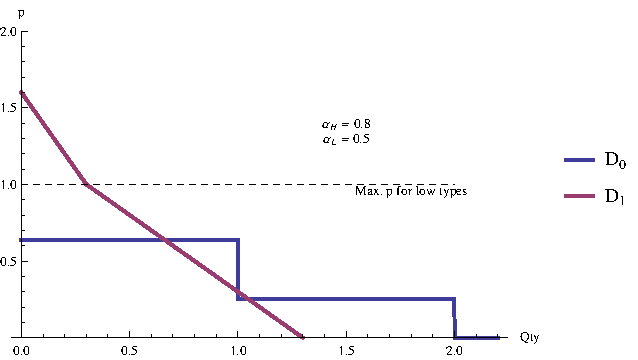
\includegraphics[scale = 1]{./diagrams/p2plr_demand.pdf}
\end{figure} 

Recall that in the pre-P2P rental market with two consumer types, if $p > \alpha_H^2$, then no consumer bought the good. 
\important{Figure~\ref{fig:demand} shows this and it shows that with the P2P rental market in long-run equilibrium, demand can be non-zero above this point.}  
Intuitively, if a would-be owner can earn rental income from their unused capacity, it seems likely that a higher product market price is supportable. 
The highest possible price that can support a market pre-P2P rental is $\bar{p}_0 = \alpha_H^2$.  
In the long-run P2P market, $D(p) = \alpha_H + \alpha_L - p$, and so $\bar{p}_{1} = \alpha_H + \alpha_L$. 
\important{Since $\alpha_H > \alpha_H^2$ and $\alpha_L > 0$, $\bar{p}_1 > \bar{p}_0$: the existence of a P2P rental market can support a higher product market price.} 

In this high-price range, the $D_1$ curve is kinked at $p = 2\alpha_L$. 
\important{The reason for this kink is that if $2\alpha_L < p$, the low-types do not use the good in the long-run P2P equilibrium.} 
The reason is simple: if $p > 2\alpha_L$, usage of the good offers negative utility from any amount of usage and so the low-types use none. 
If $p > 2 \alpha_L$, then the long-run P2P equilibrium is one in which the high-types simply trade with themselves, creating a market demand of just $D(p) = \alpha_H - p/2$. 
\important{The model suggests the possibility of a transitory short-run phase in which low-types get access that disappears once former-owners become renters and bid up rental rates.} 

\subsection{Long-run P2P rental market consumer surplus when both consumer types use the good} 
If both high- and low-types participate in the long-run P2P equilibrium, social surplus (assuming no price changes in the product market) is 
\begin{align} 
S_1 & = \frac{1}{4}(p - 2\alpha_H)^2 + \frac{1}{4}(p - 2\alpha_L)^2 \notag \\
    & = \alpha_H^2 + \alpha_L^2 - p(\alpha_H + \alpha_L) + \frac{p^2}{2} \notag 
\end{align} 
whereas in the pre-P2P rental market, surplus was $S_0 = \alpha_H^2 - p$.  
The long-run social surplus from the introduction of the P2P rental market is  
\begin{align}
\Delta S = S_1 - S_0 = \alpha_L^2 + (1 - \alpha_L - \alpha_H)p + p^2/2.  
\end{align} 
From the requirement that $\alpha_L^2 < p < \alpha_H^2$ and the assumption that the low-types use some of the good in equilibrium ($2 \alpha_L > p$), we can show that $\Delta S > 0$. 
\important{We can also show that social surplus from the long-run P2P rental market is increasing the low-type valuation, or $\Delta S'(\alpha_L) > 0$, again because $2\alpha_L > p$.}
\important{For the high-types, $\Delta S'(\alpha_H) = -p < 0$, and so the social surplus from sharing is 
reduced when the high-types have a higher valuation (as was the case in the short-run).}

% \section{Continuous Types Model} 
% Assume that $\alpha \sim U[0,1]$. 
% Each consumer---if they consume at all---consumes $x_i = \alpha_i - r/2$. 
% The consumer indifferent between purchasing and not has $\bar{\alpha} = \sqrt{p}$. 
% At a rental rate of $r$, only those with $\alpha > r/2$ consumer any of the good. 
% Let $\underline{\alpha} = r/2$. 
% Short-run market clearing is thus: 
% \begin{align}
% \int_{\underline{\alpha}}^{\bar{\alpha}} x(\alpha, r)\,d\alpha = \int_{\bar{\alpha}}^1 \left( 1 - x(\alpha,r) \right)  \,d\alpha
% \end{align} 
% and so 
% \begin{align} 
% r^* = 2 \left(1-\sqrt{2} \sqrt{1-\sqrt{p}}\right).
% \end{align} 
% For $p \le \frac{1}{4}$, $r^* \le 0$. 

% \begin{figure}
% \centering
% \caption{Comparison of long- and short-run rental rates as a function of market-clearing price} 
% \begin{minipage}{0.80 \linewidth}
% 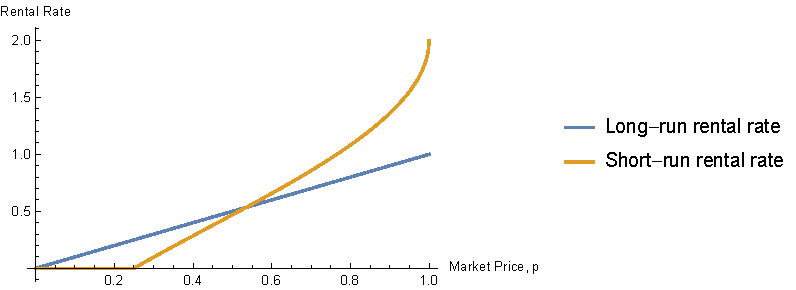
\includegraphics{./plots/cont_types.pdf}
% \end{minipage}
% \end{figure} 

% \begin{figure}
% \centering
% \caption{Quantity exchanged} 
% \begin{minipage}{0.80 \linewidth}
% 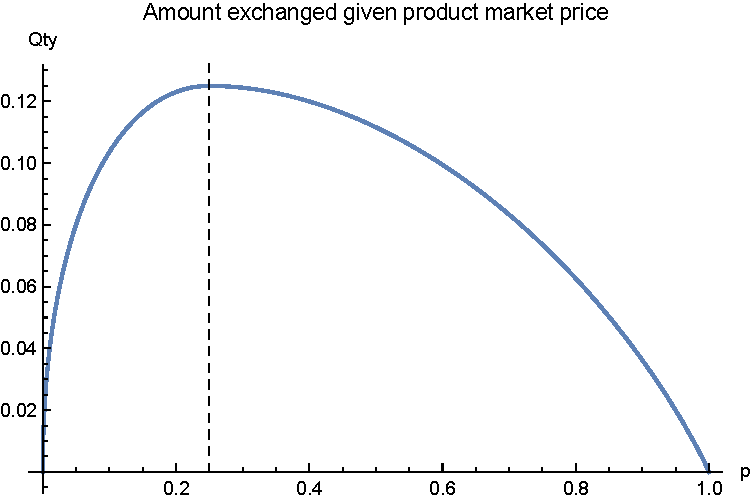
\includegraphics{./plots/cont_qty.pdf}
% \end{minipage}
% \end{figure} 

\section{The attributes of goods and the feasibility of renting} 
In the model, a good is described by several parameters: the purchase price, $p$, the usage valuation, $\alpha$, and, if we consider transaction costs, $c$.  
If we look to what goods are currently commonly rented now, we get a sense of what makes something amenable to renting: 
relatively low $\alpha$, high $p$ and low $c$, or expensive goods that are used infrequently but predictably and are not wholly consumed by usage. 
Examples include cars and hotels in distant cities, tuxedos, certain kinds of specialty tools (e.g., rototillers, carpet shampooers) and so on. 
The conditions necessary for the P2P rental market are similar, except that we also need a stock of owners and non-owners. 

When product market prices are so low that nearly everyone buys the product, no P2P rental market can exist even when total usage is low.  
For example, there is no rental market in kitchen timers---although they are used infrequently and quite durable, there is neither supply (owning consumers would not find it worth the hassle to rent them out) nor demand (if a consumer wants one, they go to the product market and buy one). 
Other goods are expensive, but there is no excess capacity, as they are used more or less continuously, giving no spare capacity: this is why there is no P2P rental market in prescription eyeglasses. 

Even at constant total amounts of usage, goods differ in the granularity of typical usage: 
a person might use their vacation home in week-long chunks of time, their lawn-mower in hour-long chunks and their tooth brush in minute-long chunks. 
These usage chunks also differ in their predictability. 
Some goods have a highly predictable usage pattern---a family might arrange to rent a vacation home months in advance---whereas other goods are much less predictable in their normal pattern of usage---the need for a back-up electric generator is almost always a surprise.  
It seems likely that goods with predictable (and easily adjustable), ``large chunk'' usage patterns should be more amenable to P2P rental markets than goods with unpredictable, granular usage patterns. 

Predicting what goods are profitably amenable to P2P rental is a task best left to entrepreneurs. 
However, it is still useful to get a sense of where these markets might evolve by surveying consumers. 
One interesting source of market sentiment about P2P rental comes from Google, which will ``auto-complete'' partial queries, providing a proxy for what other Google users are search for. 
Figure~\ref{fig:auto} shows the ``auto-suggest'' query completions from the Google Search toolbar for the partial query ``Airbnb for.''
Some of the queries are easy to understand: 
cars, office space, parking, boats, storage, event space and bikes are all indeed goods for which there are already P2P rental markets. 
The phrase ``airbnb for dogs'' likely means kennel space and dog boarding, not rental dogs, while ``airbnb for food'' likely means services where chefs will come to your house to cook, ala KitchenSurfing. 
And ``Airbnb for ipad'' is presumably the result of individuals looking for that iPad application made by Airbnb. 

\begin{figure}
\centering 
\caption{Google Auto-Suggest for ``Airbnb for '' Partial Query}
\label{fig:auto} 
\begin{minipage}{0.80 \linewidth}
 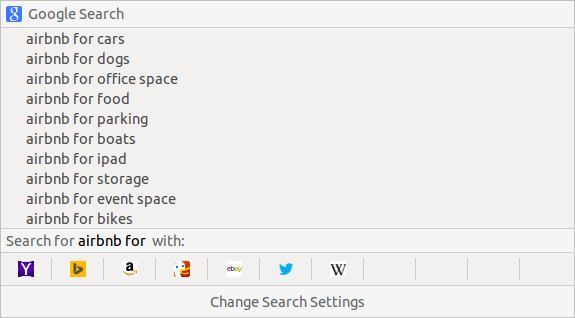
\includegraphics[width = \linewidth]{./images/airbnb_for_x.png}
\end{minipage}
\end{figure} 

To move beyond the casual empiricism of considering what P2P rental markets might exist (or not) for various goods, we conducted a consumer survey on Amazon Mechanical Turk. 
The survey focused on consumer decision-making and usage patterns for a variety of goods. 
Although MTurk offers a convenience sample, there is no strong reason to think they would have highly idiosyncratic consumption patterns. 
Furthermore, for our purposes, the MTurk population is useful for two reasons. 
First, because it is easy to pay for small amounts of work, it is easy to keep incentives high for even a very long survey. 
Second, because the MTurk population is willing---and has incentives to---carefully answer a tedious set of questions, they are less likely to quickly and carelessly complete the survey; 
workers on MTurk who have their work ``rejected'' by dissatisfied employers become ineligible for the best, highest-paying kinds of work on the marketplace and as such show a high level of diligence.    
This respondent diligence makes it useful for certain kinds of questions (for example, \cite{kuziemko2013elastic} used the MTurk population to study elasticities of demand for redistribution).  

\subsection{Design and administration of the survey}
We hired US-based ``Master'' workers to answer a questions about a consumer good, e.g., BBQ grill, pick-up truck, men's suit, toothbrush etc.
We asked questions about a total of 26 goods that we selected because we thought they would yield interesting answers and had some variation in purpose (e.g., recreation, home improvement, cooking and so on), purchase price, predictability and granularity. 
We asked them: whether they owned the good; whether they had ever rented or lent out the good; how much they would use the good \emph{regardless} of whether they actually owned the good; whether they would use the good in one large chunk or many small chunks; whether usage was predictable; why they did not own the good; and finally, what was their household income. 
See Appendix~\ref{sec:survey} for the full list of goods as well as the actual survey questions and answers.  
Each ``human intelligence task'' or HIT was a total of eight questions about one particular good, with one question about family income. 
Workers were allowed to answer for each of the 20 goods.  
 
\subsection{Ownership and renting patterns} 
For each good, the respondent was asked whether their household owns such a good. 
Figure~\ref{fig:frac_owning} shows the fraction of respondents reporting owning various goods, as well as 95\% confidence intervals for that point estimate computing using the Wilson method for a binary proportion.    
There are few surprises: nearly everyone owns a toothbrush, a hammer and a blender; no one reported owning a jet ski and only one respondent reported owning a vacation home.
Figure~\ref{fig:frac_renting} shows the fraction of respondents reporting having rented the various goods. 
\important{Generally, ownership and renting appear to be gross substitutes, with the notable exception of cars, presumably because people rent cars when traveling.}

\begin{figure}
\centering 
\caption{Fraction of respondents owning various goods \label{fig:frac_owning} }
\begin{minipage}{0.90 \linewidth}
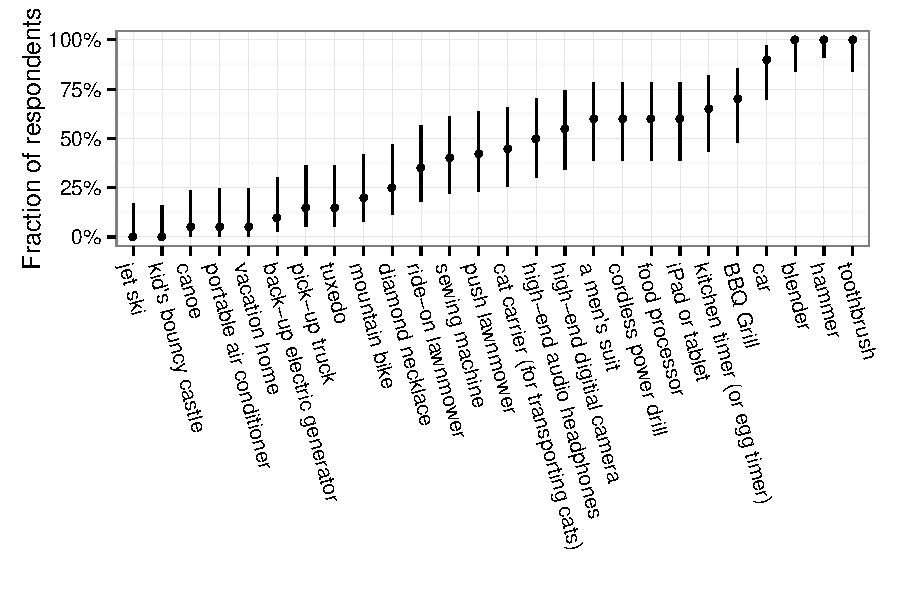
\includegraphics[width = \linewidth]{./plots/ownership_fractions.pdf} 
\end{minipage} 
\end{figure} 

\begin{figure}
\centering 
\caption{Fraction of respondents reporting having rented various goods \label{fig:frac_renting}}
\begin{minipage}{0.90 \linewidth}
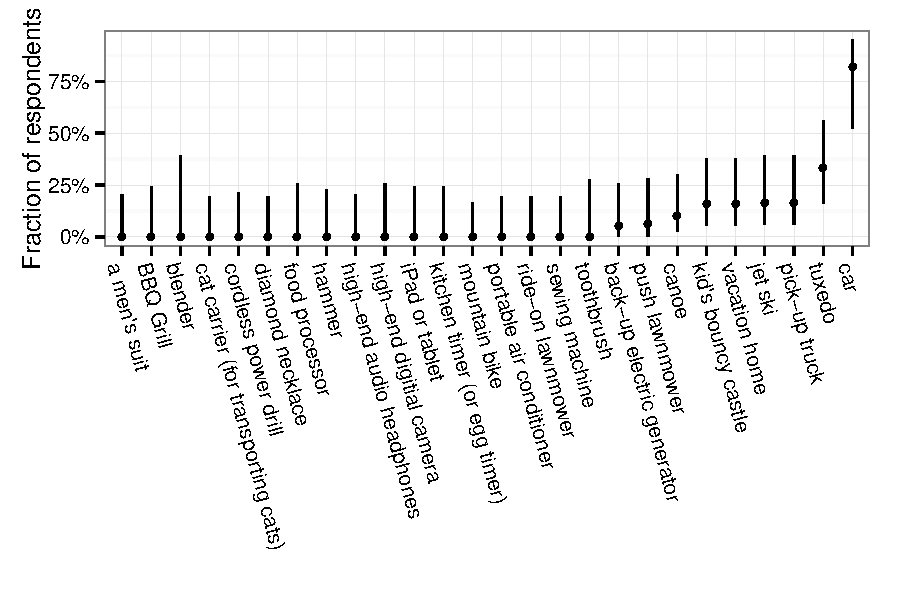
\includegraphics[width = \linewidth]{./plots/rental_fractions.pdf} 
\end{minipage} 
\end{figure} 

Figure~\ref{fig:scatter} plots the fraction of respondents reporting having rented a good versus the fraction owning, with both axes on a square-root scale.  
There is generally a negative relationship between owning and renting. 
Goods that are used during special occasions like weddings, celebrations and vacations show the highest rates of rental and lowest rates of ownership, e.g., tuxedos, vacation homes, jet ski, tuxedos, canoes, bouncy castles. 
There may also be some evidence of expensive tools useful for one-off jobs being rented, such as an electric generator and a pick-up truck. 
Unsurprisingly, goods with nearly universal ownership show little renting with the notable exception of cars, which are both owned and rented at high rates.  
\important{There are a number of goods (not all labeled) that show medium ownership levels (e.g., around 50\%) and yet zero recorded instances of renting.} 

To confirm the visual pattern of renting declining in ownership, we report the results of two OLS regressions of the form
\begin{align}
\textsc{FracRent}_g = \beta_0 + \beta_1 \textsc{FracOwn}_g + \epsilon,  
\end{align} 
where $\textsc{FracOwn}_g$ is the fraction of respondents claiming to own good $g$ and $\textsc{FracRent}_g$ is the faction claiming to have rented good $g$. 
Table~\ref{tab:own_vs_rent} reports the estimated regression of this equation, with cars included in Column~(1) and cars excluded in Column~(2). 
\important{If we exclude cars, there is a strong negative relationship between owning and renting.}


\begin{figure}
\centering 
\caption{Fraction renting versus fraction owning \label{fig:scatter} }
\begin{minipage}{0.60 \linewidth}
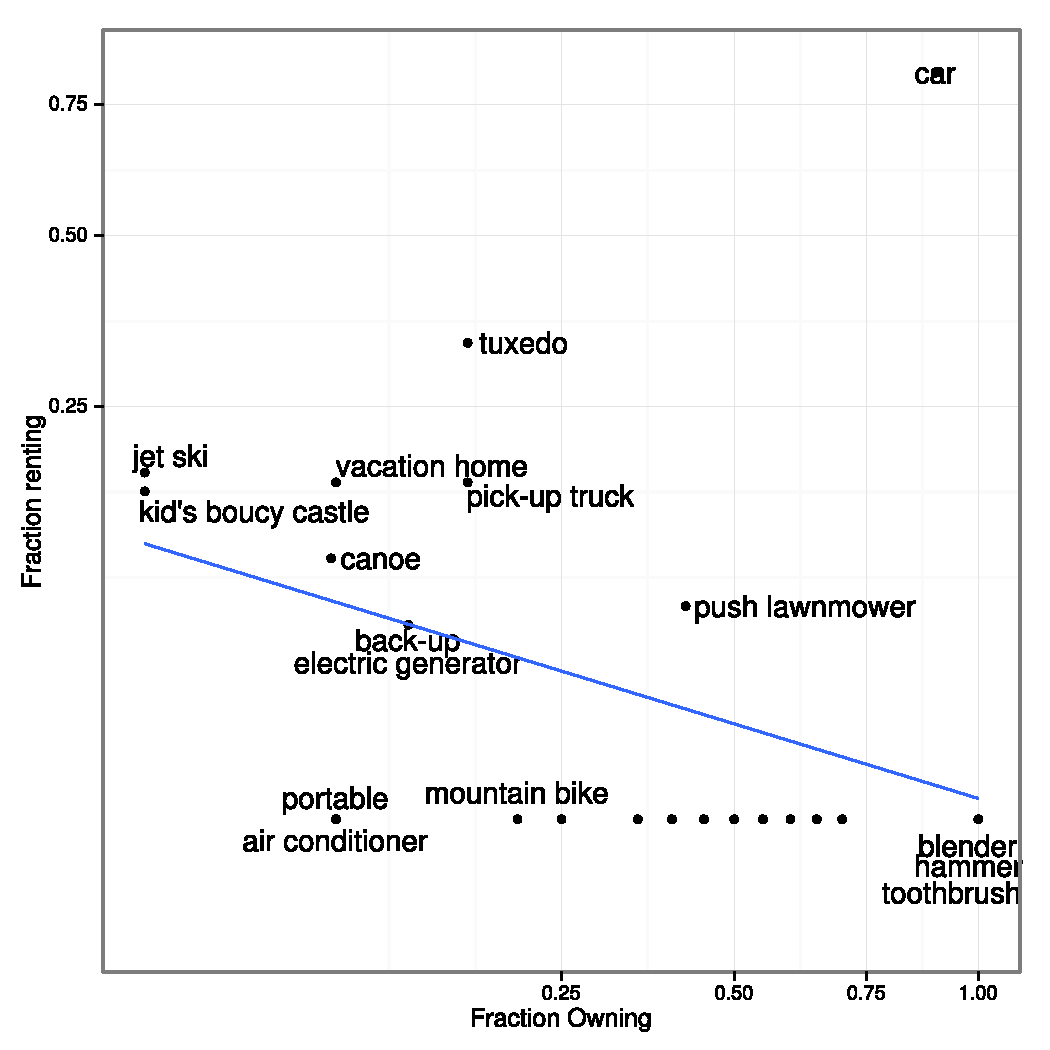
\includegraphics[width = \linewidth]{./plots/scatter_rent_v_own.pdf} 
\end{minipage} 
\end{figure} 


% Table created by stargazer v.5.2 by Marek Hlavac, Harvard University. E-mail: hlavac at fas.harvard.edu
% Date and time: Tue, Jan 26, 2016 - 07:25:21 AM
% Requires LaTeX packages: dcolumn 
\begin{table}[!htbp] \centering 
  \caption{Fraction of respondents owning a good versus fraction having rented a good} 
  \label{tab:own_vs_rent} 
\footnotesize 
\begin{tabular}{@{\extracolsep{5pt}}lD{.}{.}{-3} D{.}{.}{-3} } 
\\[-1.8ex]\hline 
\hline \\[-1.8ex] 
 & \multicolumn{2}{c}{\textit{Dependent variable:}} \\ 
\cline{2-3} 
\\[-1.8ex] & \multicolumn{2}{c}{Fraction reporting renting the good (\textsc{FracRental})} \\ 
\\[-1.8ex] & \multicolumn{1}{c}{(1)} & \multicolumn{1}{c}{(2)}\\ 
\hline \\[-1.8ex] 
 Fraction reporting owning the good & -0.009 & -0.160^{***} \\ 
  & (0.109) & (0.046) \\ 
  Constant & 0.081 & 0.115^{***} \\ 
  & (0.059) & (0.024) \\ 
 \hline \\[-1.8ex] 
Sample & \multicolumn{1}{c}{All Goods} & \multicolumn{1}{c}{Cars Excluded} \\ 
Observations & \multicolumn{1}{c}{26} & \multicolumn{1}{c}{25} \\ 
R$^{2}$ & \multicolumn{1}{c}{0.0003} & \multicolumn{1}{c}{0.345} \\ 
\hline 
\hline \\[-1.8ex] 
\end{tabular}
\\{\footnotesize \begin{minipage}{0.85 \linewidth} \emph{Notes:}
The unit of observation for the regressions in this table is the individual good.
The dependent variable is the fraction of respondents reporting having rented that good, while the independent variable is the fraction reporting owning that good. 
Column~(1) includes all goods surveyed, while Column~(2) excludes cars.
For the full list of goods and the survey language, see Appendix~\ref{sec:survey}. 
\starlanguage \end{minipage} }
\end{table}


\subsection{Ownership and usage} 
In the model, consumers considered how much they would use some good and then compared the resultant usage utility against the purchase price. 
The model predicts increasing ownership in estimated usage. 
To elicit usage, we asked respondents to select how often they would use a good in time units, using familiar measures of time to label the responses e.g., 1 hour a week, 1 hour a day and so on.
We framed the choices as being approximately on a logarithmic scale, with each increase in usage being approximately a doubling of the fraction of time. See Appendix~\ref{sec:survey} for the actual choices.   

In Figure~\ref{fig:ownership_distro}, we plot the kernel density estimates of log usage (as fractions of time) for owners and non-owners, with those reporting no usage at all excluded. 
Because ownership fractions differ substantially across goods, a density estimate is not always possible for both owners and non-owners. 
Even when a density is, one is often far less precise than the other. 
For some goods with both distributions, there does seem to be a right-shifted usage distribution among owners: 
the power drill, the diamond necklace, the high-end headphones, the mountain bike, the pick-up truck and perhaps the sewing machine. 
However, the food processor and perhaps the tablet and the push lawn-mowers show an alternate pattern. 
This graphical approach makes it difficult to identify meaningful differences and it fails to account for income effects. 

\begin{figure}
\centering 
\caption{Usage by ownership, by good \label{fig:ownership_distro}}
\begin{minipage}{0.90 \linewidth}
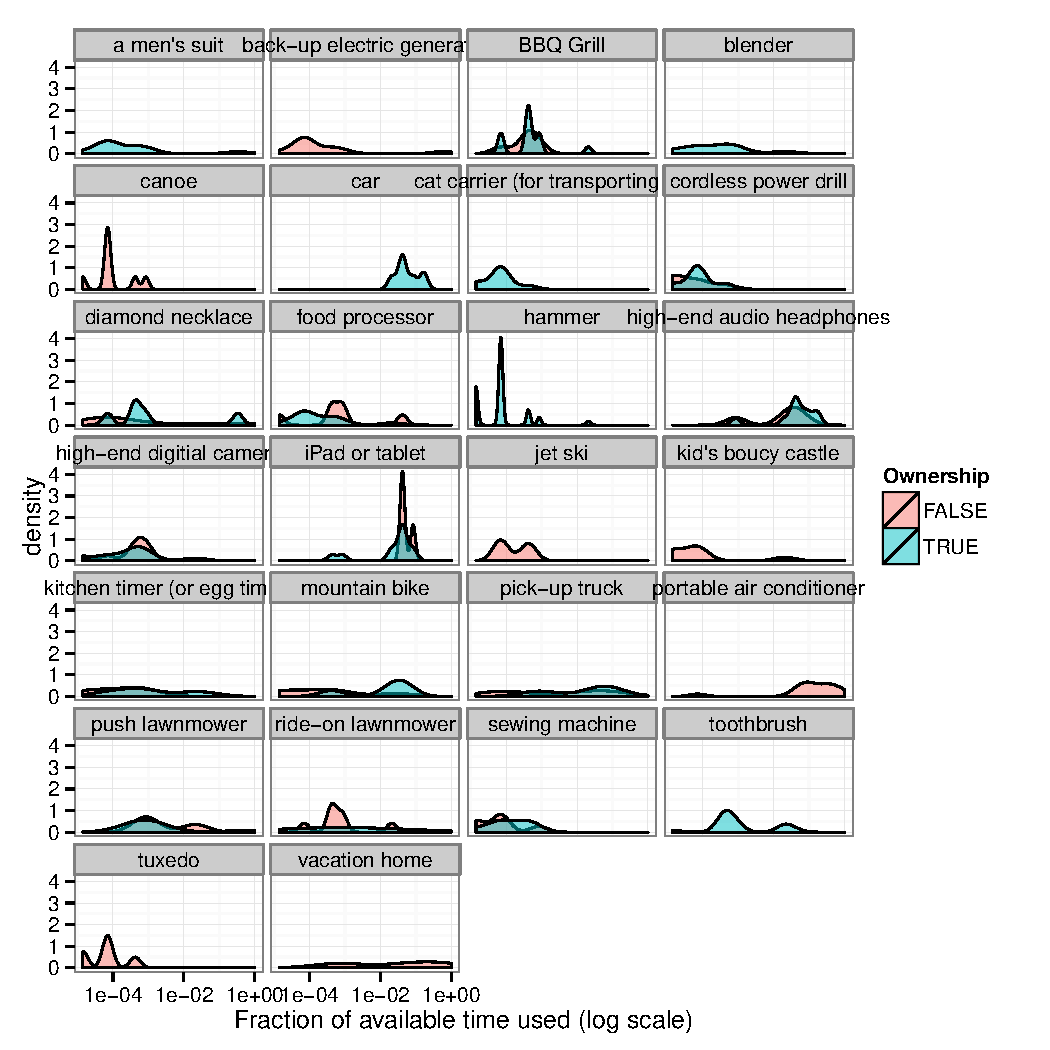
\includegraphics[width = \linewidth]{./plots/ownership_distro.pdf} 
\end{minipage} 
\end{figure} 

To explore the usage/ownership relations further, we regress ownership on self-reported usage measures. 
In Column~(1) of Table~\ref{tab:ownership}, we report a regression where the ownership indicator for respondent $i$ owning good $g$  is regressed upon the log fraction of usage, $\log x_{ig}$ (replaced by $0$ in the design matrix when $x_{ig} = 0$ and an indicator for zero reported usage, $\mathbb{1}\cdot\{x_{ig} = 0\}$:  
\begin{align} \label{eq:base_own}
\textsc{Own}_{ig} = \beta_0 + \beta_1 \log x_{ig} + \beta_2 \mathbb{1}\cdot\{x_{ig} = 0\} + \mu_{g} + \epsilon_{ig}.
\end{align} 
where $\mu_g$ is a good-specific effect. 
This effect is random in Column~(1) and fixed in Column~(2).
Aside from the difficulty in transforming a highly-skewed $x$ distribution that contains zero, treating the $x = 0$ case separately with its own indicator seems sensible in our context, as this response is qualitatively different from the other answers. 

We can potentially get a more precise estimate of the effects of usage differences on ownership by controlling for some other sources of variation in ownership. 
First, the nature of the good affects the probability of ownership independent of the respondent's estimated usage. 
Second, different goods presumably have different income elasticities.  
To capture these sources of variation, in Column~(3), we report an estimate of 
\begin{align} \label{eq:usage_and_income}
\mbox{own}_{ig} = \beta_0 + \beta_1 \log x_{ig} + \beta_2 1\cdot\{x_{ig} = 0\} + \mu_g + \beta_g \mbox{IncomeIndex}_i + \epsilon_{ij}  
\end{align} 
where $\mu_g$ is a good-specific random effect and $\beta_g$ is a good-specific slope on the respondent's income index (the standardized mean of their income response---see Appendix~\ref{sec:survey} for the income bands). 


% Table created by stargazer v.5.1 by Marek Hlavac, Harvard University. E-mail: hlavac at fas.harvard.edu
% Date and time: Thu, May 14, 2015 - 07:55:45 AM
% Requires LaTeX packages: dcolumn 
\begin{table}[!htbp] \centering 
  \caption{Respondent estimates of the fraction of time spent using a good and whether they own that good} 
  \label{tab:ownership} 
\footnotesize 
\begin{tabular}{@{\extracolsep{5pt}}lD{.}{.}{-3} D{.}{.}{-3} D{.}{.}{-3} } 
\\[-1.8ex]\hline 
\hline \\[-1.8ex] 
 & \multicolumn{3}{c}{\textit{Dependent variable:}} \\ 
\cline{2-4} 
\\[-1.8ex] & \multicolumn{3}{c}{Respondent owns the item?, ($\textsc{Own}_{ig}=1$)} \\ 
\\[-1.8ex] & \multicolumn{1}{c}{(1)} & \multicolumn{1}{c}{(2)} & \multicolumn{1}{c}{(3)}\\ 
\hline \\[-1.8ex] 
 Log estimated usage, $\log x_{ig}$ & 0.026^{**} & 0.026^{**} & 0.026^{**} \\ 
  & (0.011) & (0.011) & (0.011) \\ 
  Log household income, $\log y_i$ &  & 0.102^{***} &  \\ 
  &  & (0.025) &  \\ 
 \hline \\[-1.8ex] 
Good FE & \multicolumn{1}{c}{Y} & \multicolumn{1}{c}{Y} & \multicolumn{1}{c}{Y} \\ 
Respondent FE & \multicolumn{1}{c}{N} & \multicolumn{1}{c}{N} & \multicolumn{1}{c}{Y} \\ 
Observations & \multicolumn{1}{c}{411} & \multicolumn{1}{c}{411} & \multicolumn{1}{c}{411} \\ 
R$^{2}$ & \multicolumn{1}{c}{0.445} & \multicolumn{1}{c}{0.465} & \multicolumn{1}{c}{0.567} \\ 
\hline 
\hline \\[-1.8ex] 
\end{tabular}
\\{\footnotesize \begin{minipage}{0.75 \linewidth} \emph{Notes:}
This table reports OLS regressions where the dependent variable is an indicator for whether a respondent reported owning a particular good.
In Column~(1) the independent variable is that respondent's estimate of what fraction of their time they would spend using that good (in logs).
In Column~(2) a regressor for the log of the respondent's self-reported household income is added to the Column~(1) specification.
Column~(3) uses the same specification as Column~(1), but a respondent specific fixed effect is added. 
The sample is restricted to respondents who reports some positive amount of predicted usage of the good and reported their household income.
All regressions include good-specific fixed effects and standard errors are clustered at the good level. 
\starlanguage \end{minipage} }
\end{table}


\important{As the model predicts, higher estimated usage predicts ownership, even when we exclude individuals who said they would have not used the good at all.} 
The coefficient on log usage is approximately the same across specifications, with somewhat more precise estimates afforded by controlling for income. 
As we would expect, individuals claiming they would not use the good at all are far less likely to own the good. 
While it increases precision, accounting for income effects as in Column~(3) seems to have little effect on the estimates. 
The absence of strong income effects is puzzling, as some of the goods in question are clearly normal goods (e.g., high-end audio headphones). 
We can partially investigate this finding by examining by good the reasons given for non-ownership. 

In the survey, non-owners were asked for there reasons for not owning the good:
``If you do not own a {\bf good}, what is the primary reason?''
\begin{itemize} 
\item NA - we own one.
\item We wouldn't use it enough to justify the purchase price
\item We would use it, but we simply do not have the money.
\item I don't have the space for this item
\end{itemize} 
Figure~\ref{fig:reasons} shows the fraction of respondents selecting among the reasons given for non-ownership of a good. 
For each point estimate, a 95\% confidence interval is shown using the Wilson method. 
The only goods where income-effects are the primary explanation (and non-ownership is not trivial) are the car, the audio headphones, and the vacation home (strongly so). 
In nearly all the other goods, the response about too little usage to justify the purchase was paramount. 
Interestingly, the goods that to date have seen the most successful P2P rental markets emerge are those for cars (e.g., RelayRides, UberX) and housing (Airbnb). 

\begin{figure}
\centering 
\caption{Reasons given for non-ownership} 
\label{fig:reasons}
\begin{minipage}{0.90 \linewidth}
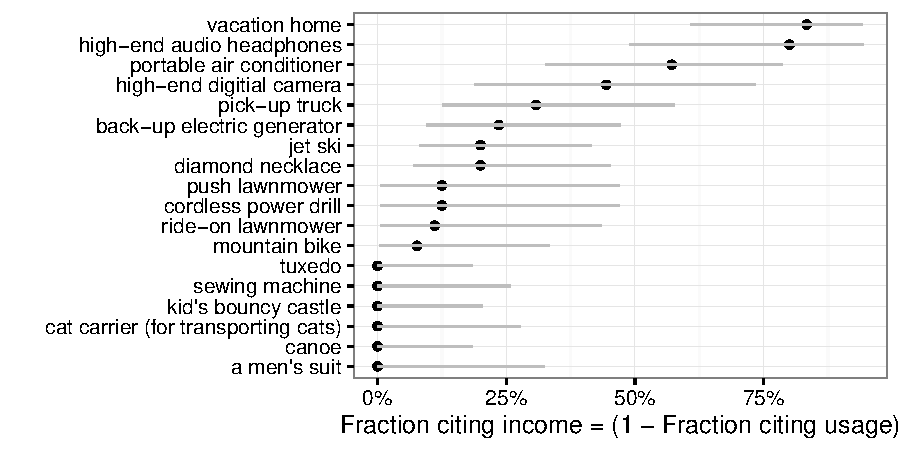
\includegraphics[width = \linewidth]{./plots/reasons.pdf} 
\end{minipage} 
\end{figure} 

\subsection{Good attributes and usage patterns} 
In addition to price and planned usage, goods differ in the predictability and granularity of that usage.
Goods with highly predictable usage patterns might be easier to rent (or lend out), whereas goods that have unpredictable usage patterns would be difficult to rent out without substantial utility loss to the owner.
Similarly, for goods that are used in numerous small sessions, renting
or lending out the good to others would create high transaction costs.
Respondents were asked to rate the unpredictability of usage on a 1-5 scale (1 was highly predictable and 5 was highly unpredictable) as well as granularity (1 was low granularity---one big chunk--- and 5 was high granularity---lots of little chunks).  

The mean unpredictability scores by good seem sensible: 
Figure~\ref{fig:predict_index} shows the mean unpredictability index per good. 
The most predictable goods are either those associated with planned recreation (e.g., vacation home, canoe, jet ski, tuxedo) or predictable chores (e.g., toothbrush, the two kinds of lawnmowers). 
The most unpredictable goods are associated with either food preparation (e.g., blender, food processor) or repairs (e.g., hammer, sewing machine, cordless power drill). 
Back-up electric generator is a clear (and unsurprising) outlier---you are in a sense always ``surprised'' when you need to use it. 

\begin{figure}
\centering 
\caption{Mean unpredictability index by good \label{fig:predict_index} }
\begin{minipage}{0.90 \linewidth}
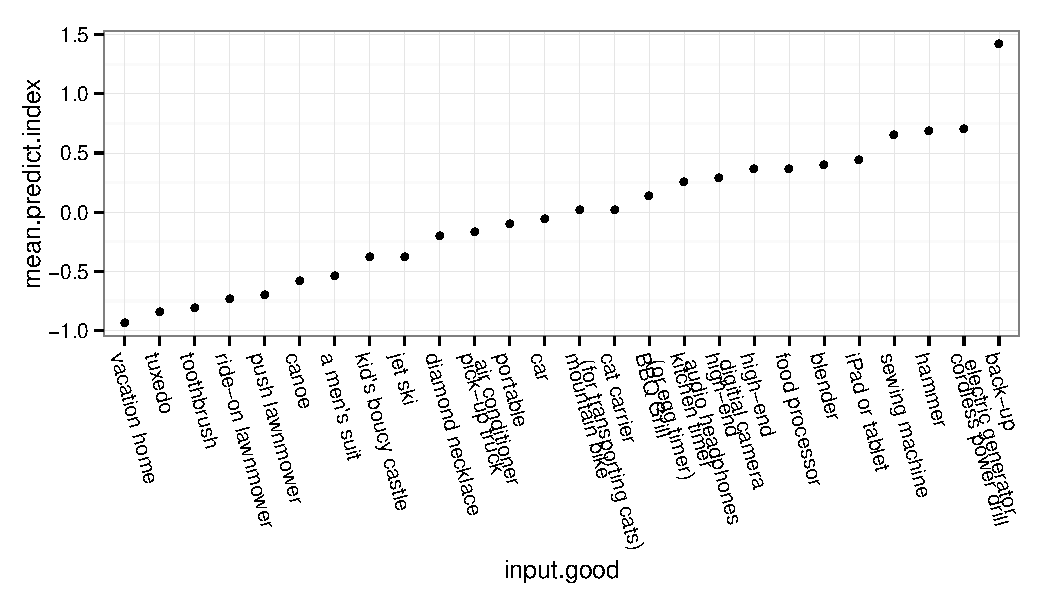
\includegraphics[width = \linewidth]{./plots/predictability.pdf} 
\end{minipage} 
\end{figure} 

Figure~\ref{fig:granularity} shows the mean granularity index per good. 
There appears to be some similarity in high predictable usage, but some goods with very granular usage also appear to have highly predictable usage---namely the toothbrush. 
To make this relationship explicit, in Figure~\ref{fig:granularity_v_predictability} the granularity and unpredictability indices are plotted against each other. 
\important{With the exception of two goods---the toothbrush and back-up generator---unpredictability and granularity are strongly positively correlated.}

\begin{figure}
\centering 
\caption{Mean granularity index by good \label{fig:granularity}}
\begin{minipage}{0.90 \linewidth}
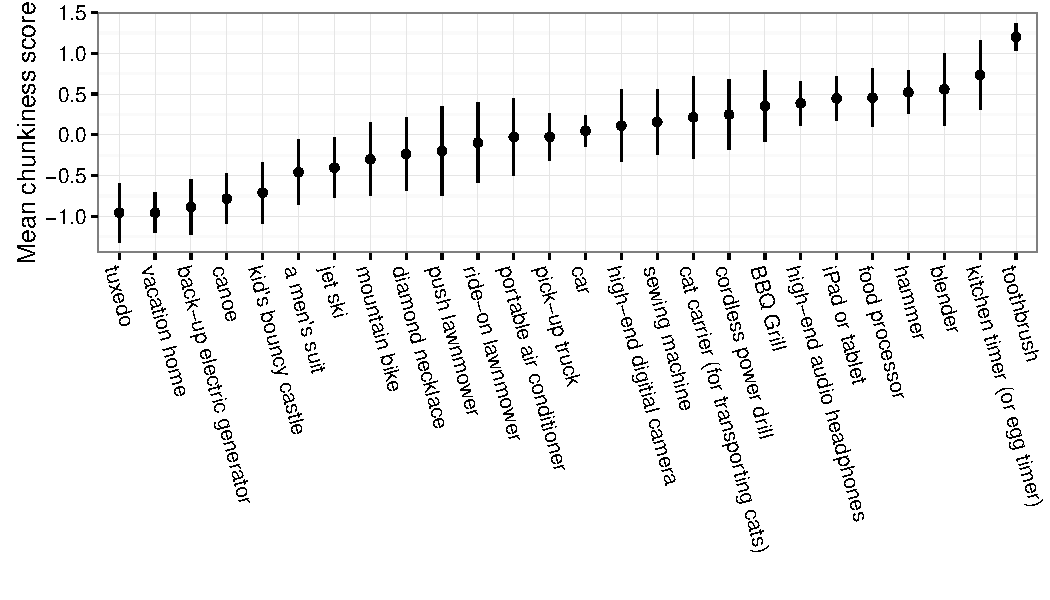
\includegraphics[width = \linewidth]{./plots/granularity.pdf} 
\end{minipage} 
\end{figure} 

\begin{figure}
\centering 
\caption{Usage predictability versus granularity \label{fig:granularity_v_predictability}}
\begin{minipage}{0.60 \linewidth}
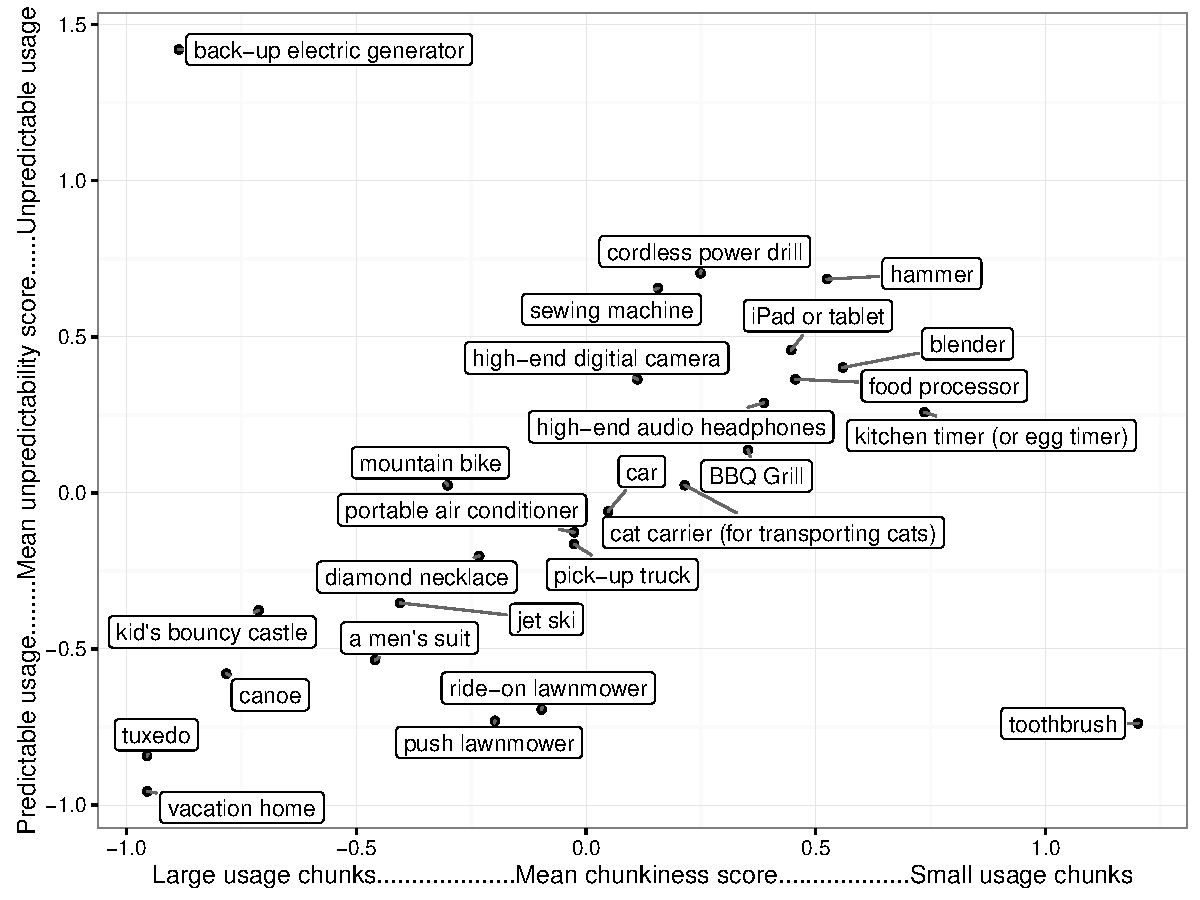
\includegraphics[width = \linewidth]{./plots/granularity_versus_predictability.pdf} 
\end{minipage} 
\end{figure} 

To test whether these unpredictability/granularity measures are related to ownership, in Table~\ref{tab:ownership_attr}, we report regressions of the ownership decision on the respondent's granularity and unpredictability scores. 
We include worker-specific random-effects in each regression. 
\important{Goods with unpredictable and highly granular usage are substantially more likely to be owned.}
In Column~(1), we see that the less predictable perceived usage, the more likely the good is to be owned. 
In Column~(2), the more granular usage is, the more likely the good it to be owned. 
Column~(3) shows that both measures still have a positive relationship with ownership but that there is no strong interaction effect between the two measures. 


% Table created by stargazer v.5.2 by Marek Hlavac, Harvard University. E-mail: hlavac at fas.harvard.edu
% Date and time: Tue, Jan 26, 2016 - 07:25:30 AM
% Requires LaTeX packages: dcolumn 
\begin{table}[!htbp] \centering 
  \caption{Good usage unpredictability and chunkiness and its association with good ownership.} 
  \label{tab:ownership_attr} 
\footnotesize 
\begin{tabular}{@{\extracolsep{5pt}}lD{.}{.}{-3} D{.}{.}{-3} D{.}{.}{-3} D{.}{.}{-3} } 
\\[-1.8ex]\hline 
\hline \\[-1.8ex] 
 & \multicolumn{4}{c}{\textit{Dependent variable:}} \\ 
\cline{2-5} 
\\[-1.8ex] & \multicolumn{4}{c}{Item is owned} \\ 
\\[-1.8ex] & \multicolumn{1}{c}{(1)} & \multicolumn{1}{c}{(2)} & \multicolumn{1}{c}{(3)} & \multicolumn{1}{c}{(4)}\\ 
\hline \\[-1.8ex] 
 Unpredictability Score (US) & 0.139^{***} &  & 0.095^{***} & 0.003 \\ 
  & (0.030) &  & (0.034) & (0.034) \\ 
  Chunkiness Score (CS) &  & 0.135^{***} & 0.091^{***} & -0.018 \\ 
  &  & (0.025) & (0.029) & (0.025) \\ 
  US x CS &  &  & -0.009 & 0.006 \\ 
  &  &  & (0.018) & (0.018) \\ 
 \hline \\[-1.8ex] 
Respondent FE & \multicolumn{1}{c}{Y} & \multicolumn{1}{c}{Y} & \multicolumn{1}{c}{Y} & \multicolumn{1}{c}{Y} \\ 
Good FE & \multicolumn{1}{c}{N} & \multicolumn{1}{c}{N} & \multicolumn{1}{c}{N} & \multicolumn{1}{c}{Y} \\ 
Observations & \multicolumn{1}{c}{489} & \multicolumn{1}{c}{489} & \multicolumn{1}{c}{489} & \multicolumn{1}{c}{489} \\ 
R$^{2}$ & \multicolumn{1}{c}{0.170} & \multicolumn{1}{c}{0.169} & \multicolumn{1}{c}{0.191} & \multicolumn{1}{c}{0.500} \\ 
\hline 
\hline \\[-1.8ex] 
\end{tabular}
\\ {\footnotesize  \begin{minipage}{0.85 \linewidth} \emph{Notes:}
This table reports regressions of an indicator for whether the respondent owns a good on that same respondent's estimates of the unpredictability and granularity of usage for that good.
The two indices are normalized responses to the 1-5 scale questions on usage chunkiness and unpredictability, pooled over all respondents and goods.
Toothbrushes and backup generators are excluded from the sample. 
See Appendix~\ref{sec:survey} for the actual survey language and responses.
In each regression, a respondent-specific fixed effect is included.
Standard errors are clustered at the level of the individual respondent.
\starlanguage
\end{minipage} }
\end{table}
 

The model and the survey are designed to complement each other in two ways. 
First, the survey provides justification for some of the modeling conventions, such as making planned usage the primary explanation for the pattern of ownership rather than ``taste'' or income. 
This is not to say that income effects do not matter when explaining purchases, but rather that they appear secondary.
Second, the survey offers a partial decomposition of the non-specific ``transaction costs'' that would make a good difficult or easy to share.  
P2P rental markets are now possible in part because technology has reduced transaction costs, but such markets have not emerged for all goods. 
The survey results suggest that those goods with unpredictable and highly granular usage might not support a P2P rental market even if the total usage is small. 
However, it also suggests that innovations that make usage more predictable might change this calculus. 

\section{Conclusion} 

By considering a single good in isolation, our model fails to capture what might be an important benefit of P2P rental markets: they might diversify consumption. 
Rather than buy a single good, consumers might rent a variety of goods that are horizontally differentiated.   

One long-term reaction to the rising of P2P rental markets is that firms might change the goods that they offer. 

One area where P2P rental markets could have a long-term effect is on the diversity of goods consumed. 
Consider that in some formulations of the consumer problem, consumers consume some positive amount of every good offered.
This is obviously a large departure from empirical reality if we draw fine-grained distinctions between ``goods.'' 
For example, Amazon.com currently lists 6,238 results for ``blender'' in the Home \& Kitchen category: 
presumably most households own far fewer than this, with most owning one or none.\footnote{As of October 8th, 2014.}
The reason for this pattern in the language of this model is clear: 
a consumer's $\alpha$ for Blender 2 \emph{conditional} upon owning Blender 1 is quite low and so another blender is not purchased.
However, if a rental market existed for both blender types, consumers could act upon their taste for diversity without owning a dozen blenders. 
Even if the blender example seems implausible, we should consider that very few consumers try to rent the car they normally drive or vacation in their hometown: presumably they diversify consumption in these cases precisely because they can. 

As P2P rental markets become commonplace, manufacturers will begin designing products more attractive for this additional purpose. 
For example, locks on cars and houses that allow remote entry will be more appealing. 
The emerging Internet-of-Things will make it easier to identify goods that are not being used at a moment in time and perhaps facilitate trade automatically. 
Similarly, technologies that make it easier to monitor usage (GPS, embedded sensors, streaming video of how they are being used and so on) should make contracting easier and reduce some of the informational asymmetries that contribute to transaction costs. 

As more of economic and social life are computer-mediated, platforms will use this information to verify the identify and reputation of buyers and sellers, further mitigating moral hazard and adverse selection.  
Even without these changes, individuals will purchase more durable goods to reduce the frequency of replacement. 
Advertisers will trumpet the rental stream income from a purchase and highlight the advantages of residual control rights. 

% \cite{ikkala2014defining}


\bibliographystyle{aer}
\bibliography{sharing.bib}

\newpage 

\appendix 

\section{Survey Questions \label{sec:survey}} 

The actual goods were: 

\begin{itemize} 
\item BBQ Grill
\item toothbrush
\item a men's suit
\item blender
\item canoe
\item car
\item cordless power drill
\item hammer
\item diamond necklace
\item food processor
\item hammer
\item cat carrier (for transporting cats)
\item high-end audio headphones
\item high-end digitial [sic] camera
\item iPad or tablet
\item jet ski
\item kid's boucy [sic] castle
\item kitchen timer (or egg timer)
\item mountain bike
\item pick-up truck
\item push lawnmower
\item ride-on lawnmower
\item tuxedo
\item vacation home
\item back-up electric generator
\item portable air conditioner
\item sewing machine
\end{itemize} 

\begin{itemize} 

\item Does your household own a {\bf good}?
\begin{itemize}
\item Yes
\item No
\end{itemize} 

\item Have you ever lent your {\bf good} to someone else?
\begin{itemize}
\item Yes
\item No
\item NA - we do not own one.
\end{itemize} 

\item Have you ever borrowed a {\bf good} from someone else?
\begin{itemize}
\item Yes
\item No
\item NA - we own one.
\end{itemize} 

\item Have you ever rented a {\bf good}?
\begin{itemize}
\item Yes
\item No
\item NA - we own one.
\end{itemize} 

\item Regardless of whether your household owns a {\bf good}, if you did own one, how much do you estimate it would be used by members of your household on average?

\begin{itemize} 
\item We would not use this at all
\item 1 minute a week (about 1 hour a year) 
\item 5 minutes a week (about 4 hours a year)
\item 1/2 an hour a week
\item 1 hour a week
\item 1/2 an hour a day
\item 1 hour a day
\item 2 hours a day
\item 4 hours a day
\item 8 hours a day
\item 16 hours a day
\item 24 hours a day (I would continuously be using this good)
\end{itemize} 


\item Regardless of whether you actually own a {\bf good}, how do you imagine it would be used if it was owned by your household (on a scale of 1 to 5): 
\begin{itemize} 
\item 1 - Used in one big block of time
\item 2  
\item 3 - Used in a mixture of large and small blocks of time
\item 4 
\item 5 - Used in many small blocks of time
\end{itemize} 

\item Regardless of whether you actually own a {\bf good}, how predictable would your usage of it be if you did own it: 
\begin{itemize}
\item 1 - Very predictable---I can plan usage many weeks in advance
\item 2  
\item 3 - Somewhat predictable 
\item 4 
\item 5 - Very unpredictable---I would never know exactly when I would need to use it until right beforehand. 
\end{itemize} 

\item If you do not own a {\bf good}, what is the primary reason?
\begin{itemize} 
\item NA - we own one.
\item We wouldn't use it enough to justify the purchase price
\item We would use it, but we simply do not have the money.
\item I don't have the space for this item
\end{itemize} 

\item What is your total household income? 
\begin{itemize} 
\item Less than \$10,000
\item  \$10,000-\$19,999
\item  \$20,000-\$29,999
\item  \$30,000-\$39,999
\item  \$40,000-\$49,999
\item  \$50,000-\$59,999
\item  \$60,000-\$69,999
\item  \$70,000-\$79,999
\item  \$80,000-\$89,999
\item  \$90,000-\$99,999
\item  \$100,000-\$149,000
\item  More than \$150,000
\end{itemize} 

\end{itemize}

\end{document} 

